\chapter{Metodología y Diseño de la Solución} \label{sec:Metodos}

En este capítulo se expone la metodología empleada y el diseño detallado e implementación de la solución planteada. Se describen los modelos y algoritmos, las técnicas de medición, la infraestructura como código, la observabilidad, y las estrategias de seguridad implementadas en el clúster Kubernetes.

\section{Diseño de la Solución}

El diseño responde directamente a las causas identificadas en el árbol de problemas: la ausencia de criterios objetivos para seleccionar el componente de red (CNI), la falta de visibilidad sobre el tráfico interno del clúster y el sobredimensionamiento de recursos que resulta de operar sin datos reales \cite{ref29}. La solución se estructura en cuatro pilares: una arquitectura de red controlada, un sistema de medición de Calidad de Servicio (QoS), un modelo de decisión multicriterio (MCDA) y una estrategia de seguridad automatizada.

\subsection{Arquitectura de Red y Topología}

El entorno de pruebas se diseñó para que el CNI sea la única variable entre ciclos de medición; el hardware, el sistema operativo, la topología y la duración de las pruebas permanecen constantes en todos los escenarios.

\subsubsection{Red underlay}

La red underlay constituye la infraestructura física sobre la que opera el clúster. Se optó por la nube pública de DigitalOcean en lugar de servidores físicos propios, ya que la homogeneidad del entorno elimina el ruido de hardware local ---variabilidad de NIC, temperatura, interferencias--- y garantiza que cualquier diferencia medida en throughput, latencia o CPU sea atribuible al CNI y no al sustrato \cite{ref2}. El aprovisionamiento se realizó mediante Terraform, herramienta de Infraestructura como Código (IaC): la configuración completa de los servidores queda descrita en archivos versionados, lo que permite reproducir el entorno de forma idéntica. Esta reproducibilidad es una condición necesaria para la validez del experimento, pues sin ella la comparación entre CNIs pierde valor probatorio \cite{ref7}.

Se utilizó K3s ---distribución liviana de Kubernetes--- con un nodo Master, datastore PostgreSQL gestionado por DigitalOcean y dos nodos Worker dedicados. El menor \emph{footprint} de K3s frente a Kubernetes estándar deja una mayor proporción de CPU y RAM disponible para el CNI, lo que aumenta la sensibilidad de las mediciones; el datastore externo elimina el punto único de fallo del plano de control sin la complejidad operativa de un clúster etcd. La topología incluye una red privada VPC para el tráfico interno entre nodos, de manera que la latencia medida dependa exclusivamente de la eficiencia del CNI y no de la variabilidad de Internet público \cite{ref8}.

\subsubsection{Red overlay y CNI evaluados}

La red overlay, implementada por el plugin CNI, provee la conectividad entre cargas de trabajo distribuidas en distintos nodos. Kubernetes no incluye esta funcionalidad por defecto y delega la elección del CNI en cada organización \cite{ref4,ref18}; esa libertad de elección, ejercida sin criterios objetivos basados en mediciones, es el problema central que aborda este trabajo.

El núcleo del diseño es la comparativa de cuatro CNI con filosofías de implementación distintas (Tabla~\ref{tab:cni-evaluados}).

\begin{table}[htbp]
\centering
\scriptsize
\caption{CNI evaluados: tecnología base, versión desplegada y enfoque.}
\label{tab:cni-evaluados}
\begin{tabularx}{\textwidth}{|Y|Y|Y|Y|}
\hline
\textbf{CNI} & \textbf{Tecnología Base} & \textbf{Versión} & \textbf{Enfoque} \\
\hline
Flannel & VXLAN (L2) & nativo K3s & Overlay sencillo de instalar; sin soporte nativo de NetworkPolicies. \\
\hline
Calico & VXLAN (DO VPC) & 3.29.1 Tigera Operator & Tigera Operator con \texttt{encapsulation: VXLAN}; políticas avanzadas L3/L4. \\
\hline
Cilium & eBPF + VXLAN tunnel & 1.16.5 & \texttt{routingMode=tunnel}, \texttt{tunnelProtocol=vxlan}; opera en el kernel con eBPF y filtrado L7 HTTP nativo. \\
\hline
Antrea & OVS (SDN) & 2.2.0 & Open vSwitch con sistema jerárquico de Tiers (Emergency $>$ SecurityOps $>$ NetworkOps $>$ Platform $>$ Application). \\
\hline
\end{tabularx}
\end{table}

Las tecnologías base de estos CNI sustentan dataplanes diferentes. \textbf{VXLAN} crea redes virtuales sobre redes físicas existentes encapsulando los paquetes originales dentro de paquetes UDP, lo que permite transportar tráfico de capa 2~\cite{ref19} sobre redes de capa 3; el costo es un \emph{overhead} de 50 bytes por paquete, que puede reducir el throughput efectivo en transferencias de paquetes pequeños \cite{ref12}. \textbf{eBPF} permite ejecutar programas de forma segura dentro del kernel de Linux; aplicado a redes, posibilita que Cilium intercepte y redirija paquetes sin copiarlos al espacio de usuario, eliminando una fuente principal de latencia \cite{ref27}. \textbf{Open vSwitch (OVS)} es un switch virtual orientado a SDN \cite{ref22} que Antrea emplea para implementar conectividad y políticas mediante un sistema de Tiers jerárquico, capaz de expresar reglas corporativas con mayor prioridad que las NetworkPolicies estándar de Kubernetes.

La selección de estos cuatro CNI no es arbitraria: cada uno aporta un punto de comparación específico y un riesgo característico a medir. Flannel actúa como línea base de conectividad sencilla, con el riesgo de carecer de \emph{enforcement} nativo de NetworkPolicies. Calico aporta madurez operativa y políticas de red en producción, con un posible costo por la evaluación de reglas. Cilium representa el uso de eBPF como mecanismo moderno de aceleración, visibilidad y políticas L7, a cambio de mayor complejidad conceptual y mayor consumo de RAM. Antrea aporta una aproximación basada en OVS y conceptos de SDN, con dependencia de componentes adicionales. En conjunto, cubren el espectro de opciones que enfrenta un equipo de operaciones real, desde la simplicidad operativa hasta las capacidades avanzadas de observabilidad y seguridad.

\subsection{Sistema de Medición de Calidad de Servicio (QoS)}

La Calidad de Servicio (QoS) cuantifica el comportamiento real de la red desde la perspectiva de las aplicaciones. El sistema de medición sigue los principios de la metrología de redes ---control de variables, reproducibilidad y representatividad estadística--- para que las diferencias observadas sean atribuibles al CNI y no al procedimiento de medición \cite{ref6}.

\subsubsection{Inyección de tráfico}

El tráfico se genera con iperf3, herramienta de referencia para pruebas de rendimiento de redes, que opera con un modelo cliente-servidor en el que un Pod emisor envía tráfico a un Pod receptor y ambos registran estadísticas detalladas de la transferencia. Para asegurar tráfico inter-nodo, el cliente y el servidor se separan mediante \texttt{podAntiAffinity} suave (\texttt{preferredDuringSchedulingIgnoredDuringExecution}, weight~100): con dos Workers disponibles, el scheduler los ubica en nodos distintos en la práctica, y la modalidad \texttt{preferred} ---en lugar de \texttt{required}--- mantiene la resiliencia ante reinicios de nodo. La ejecución se automatiza mediante CronJobs de Kubernetes, con ráfagas de tráfico TCP de 300 segundos cada 30 minutos, frecuencia que captura el comportamiento de la red en distintos momentos y compone un perfil estadístico representativo \cite{ref7}.

\subsubsection{Variables telemáticas capturadas}

El sistema de medición parte del principio de que una métrica aislada no describe la calidad de una red. La Tabla~\ref{tab:variables-qos} resume las variables capturadas, que combinan rendimiento de red, estabilidad y costo computacional; la latencia se registra en sus valores mínimo, promedio, máximo y de variabilidad (\emph{jitter}), de modo que los picos no queden ocultos por el promedio.

\begin{table}[htbp]
\centering
\scriptsize
\caption{Variables telemáticas capturadas por el sistema de medición.}
\label{tab:variables-qos}
\begin{tabularx}{\textwidth}{|Y|Y|Y|}
\hline
\textbf{Variable QoS} & \textbf{Unidad de medida} & \textbf{Relevancia} \\
\hline
Throughput (ancho de banda efectivo) & Gbps / Mbps & Capacidad efectiva de transferencia entre Pods. Herramienta: iperf3 \texttt{-J}, 300 s TCP. \\
\hline
Latencia de establecimiento TCP & ms (min/avg/max/mdev) & Costo de iniciar una comunicación entre servicios. Herramienta: script Bash con \texttt{nc -z -w 2}, 30 muestras por corrida. \\
\hline
Retransmisiones TCP & número de paquetes & Indicador de inestabilidad en el canal de encapsulamiento del CNI. \\
\hline
Costo computacional del CNI & \% CPU / MB RAM & Recursos que consume el propio CNI para procesar el tráfico; determina el impacto en el sobredimensionamiento. \\
\hline
\end{tabularx}
\end{table}

\subsubsection{Pila de observabilidad: Prometheus y Grafana}

\textbf{Prometheus} recolecta métricas mediante un modelo de \emph{scraping} periódico sobre cada nodo, registrando estadísticas de CPU, memoria, red y estado del CNI. El almacenamiento en series temporales permite correlacionar el consumo de recursos del agente CNI con los instantes exactos de las pruebas de throughput, verificando que las métricas de eficiencia reflejen el comportamiento bajo carga y no en reposo \cite{ref6}. \textbf{Grafana} constituye la capa de visualización: presenta en dashboards interactivos el throughput, la latencia, el consumo de CPU del agente y las retransmisiones TCP. Esta visibilidad permitió detectar anomalías durante las sesiones ---picos de CPU o reinicios inesperados del agente--- antes de que comprometieran la integridad de las corridas \cite{ref6}.

\subsection{Modelo de Decisión Multicriterio (MCDA)}

Para resolver la selección objetiva del CNI se diseñó un modelo de Análisis de Decisión Multicriterio (MCDA), enfoque empleado en ingeniería y economía cuando una decisión involucra múltiples factores con distinta importancia \cite{ref9}. A diferencia de una comparación basada en un único criterio ---por ejemplo, el throughput máximo---, el MCDA captura el \emph{trade-off} entre velocidad, eficiencia de recursos y capacidades de seguridad, y produce una recomendación que refleja las prioridades de cada tipo de organización.

\subsubsection{Limpieza estadística y normalización}

Antes de aplicar el modelo, los datos recolectados pasan por una limpieza estadística mediante el Rango Intercuartílico (IQR), que elimina \emph{outliers} causados por eventos externos como mantenimientos del proveedor o picos de uso compartido. Las métricas se re-escalan después mediante la fórmula min-max al intervalo $[1,\,5]$ (véase Marco Teórico, sección~\ref{cap:marco_teorico}), considerando el sentido de optimización de cada variable: en throughput, un valor mayor es mejor; en latencia, CPU, memoria y retransmisiones, un valor menor es preferible, por lo que el cociente de normalización se invierte. Este procesamiento evita que la recomendación dependa de valores atípicos o de la magnitud numérica de una métrica, y se implementa en el archivo \texttt{docs/procesador.js}.

\subsubsection{Matriz de ponderación dinámica y penalización de seguridad}

A diferencia de los modelos MCDA estáticos, el prototipo recomendador calcula los factores de ponderación dinámicamente mediante deslizadores (\emph{sliders}) que reflejan los requisitos del usuario y normalizan la suma al 100\%. Para la evaluación estructurada en este documento, se parametrizaron tres perfiles representativos de la industria (Fintech, Streaming e IoT). La Tabla~\ref{tab:pesos-mcda} ilustra la distribución porcentual resultante para las configuraciones predeterminadas de cada perfil calculadas por el motor.

\begin{table}[htbp]
\centering
\scriptsize
\caption{Matriz de factores de ponderación (pesos calculados) por perfil de la tesis.}
\label{tab:pesos-mcda}
\begin{tabularx}{\textwidth}{|Y|c|c|c|c|c|}
\hline
\textbf{Perfil / Caso de Uso} & \textbf{Latencia} & \textbf{Estabilidad} & \textbf{Throughput} & \textbf{Recursos} & \textbf{Seguridad} \\
\hline
Fintech / Seguridad crítica & 20.8\% & 24.8\% & 21.0\% & 8.1\% & 25.3\% \\
\hline
Streaming / Alto rendimiento & 27.7\% & 22.7\% & 25.1\% & 12.3\% & 12.3\% \\
\hline
IoT / Recursos limitados & 20.8\% & 19.0\% & 18.5\% & 28.0\% & 13.7\% \\
\hline
\end{tabularx}
\end{table}

La decisión base aplica la suma ponderada $P_{CNI}=\sum_{i=1}^{n}(V_i \times W_i)$, donde los valores $V_i$ se normalizan de forma continua en la escala $[1,\,5]$ utilizando escalado \emph{min-max}, y los pesos $W_i$ corresponden al perfil seleccionado. 

\textbf{Restricción no compensatoria:} Para evitar que un CNI inseguro gane por pura eficiencia computacional, el modelo impone una restricción matemática estricta. Si el perfil exige un nivel de seguridad \emph{Alto} o \emph{Muy Alto} (valor $\ge 4$ en el recomendador, como ocurre en el perfil Fintech), cualquier CNI que carezca de soporte nativo para Network Policies (ej. Flannel) sufre una penalización. Su puntaje final es multiplicado por un factor de $0.40$ (reducción del 60\%), lo que lo descarta algorítmicamente como opción viable en entornos regulados.

\subsection{Seguridad y Micro-segmentación (Zero Trust)}

En su configuración inicial, cualquier aplicación dentro del clúster puede comunicarse con cualquier otra. Las Network Policies permiten implementar el principio de \emph{Zero Trust}: conceder solo lo necesario y verificar explícitamente cada acceso \cite{ref24,ref25}. Esto reduce la superficie de ataque, ya que ante el compromiso de un Pod las políticas limitan el movimiento lateral a las rutas explícitamente autorizadas. La aplicación efectiva de estas políticas depende del CNI: si el plugin no las implementa en su plano de datos, la política existe como objeto declarativo sin producir efecto \cite{ref4,ref18}.

\subsubsection{Estrategia de Default Deny}

El diseño implementa Zero Trust en dos niveles: primero, una política de \emph{Default Deny} que bloquea todo el tráfico entrante y saliente de cada namespace; después, una habilitación selectiva que abre únicamente las comunicaciones necesarias. Sobre esta base se definieron tres casos de uso (Tabla~\ref{tab:casos-seguridad}), ejecutados sobre cada CNI que soporta Network Policies ---Calico, Cilium y Antrea---; Flannel se incluye como referencia negativa para confirmar la ausencia de \emph{enforcement} en su plano de datos.

\begin{table}[htbp]
\centering
\scriptsize
\caption{Casos de uso de seguridad implementados por CNI.}
\label{tab:casos-seguridad}
\begin{tabularx}{\textwidth}{|Y|Y|}
\hline
\textbf{Caso} & \textbf{Descripción} \\
\hline
\texttt{zero\_trust} & Default Deny: bloquea todo ingress y egress por defecto; permite solo el tráfico benchmark explícito. \\
\hline
\texttt{multi\_tier} & Reglas explícitas \texttt{frontend $\rightarrow$ backend $\rightarrow$ database} mediante label selectors. Cilium agrega CiliumNetworkPolicy L7 HTTP (solo GET/HEAD desde frontend). \\
\hline
\texttt{egress\_block} & Bloqueo de egress externo con DNS permitido; tráfico inter-pod interno habilitado. \\
\hline
\end{tabularx}
\end{table}

Dos CNI aportan diferenciadores propios. Cilium implementa filtrado HTTP nativo por método mediante \texttt{CiliumNetworkPolicy} L7 (\texttt{GET} y \texttt{HEAD} permitidos de frontend a backend; \texttt{POST}, \texttt{PUT} y \texttt{DELETE} bloqueados), directamente en eBPF y sin \emph{service mesh}. Antrea, mediante \texttt{ClusterNetworkPolicy} en el Tier \texttt{securityops}, impone reglas con prioridad sobre cualquier \texttt{NetworkPolicy} de namespace, modelando políticas corporativas obligatorias ---del tipo ISO 27001 o SOC 2--- que los desarrolladores no pueden sobrescribir.

\subsubsection{Automatización GitOps con ArgoCD}

Para preservar la efectividad de las políticas tras cambios en el sistema, se diseñó un flujo GitOps con ArgoCD. Si una política de red se elimina del clúster, ArgoCD detecta la diferencia entre el estado actual y el definido en Git y restaura el recurso automáticamente (\texttt{selfHeal: true}); los recursos eliminados del repositorio también se eliminan del clúster (\texttt{prune: true}). Esta automatización garantiza la integridad del experimento: durante las rotaciones de CNI, las políticas se restauran a su estado esperado sin intervención manual, lo que elimina una fuente potencial de sesgo en los resultados \cite{ref25}.

\subsection{Flujo Integral del Sistema}

El flujo completo de datos se organiza en cinco etapas:
\begin{enumerate}
\item \textbf{Generación de tráfico:} un CronJob activa iperf3-client cada 30 minutos (minutos 0 y 30); la anti-afinidad ubica cliente y servidor en nodos distintos.
\item \textbf{Captura de métricas:} iperf3 registra throughput, latencia TCP y retransmisiones (formato JSON, 300 s); un CronJob de latencia ejecuta 30 muestras con \texttt{nc -z -w 2} (minutos 10 y 40); Prometheus recolecta CPU y RAM del agente CNI.
\item \textbf{Extracción de recursos:} el CronJob del Resource Usage Exporter (minutos 25 y 55) consulta la API HTTP de Prometheus (\texttt{/api/v1/query\_range}) y genera archivos raw JSON, CSV, PNG y \texttt{cni\_resource\_summary.json}.
\item \textbf{Procesamiento y scoring MCDA:} \texttt{procesador.js} aplica IQR, normalización min-max y cálculo de puntajes, y genera \texttt{cni-data.json}.
\item \textbf{Visualización y recomendación:} una SPA en React consume \texttt{cni-data.json} y muestra el ranking MCDA por perfil.
\end{enumerate}

\subsection{Arquitectura por Capas}

La solución se organizó en siete capas para separar responsabilidades: la \textbf{capa 1} es la infraestructura underlay (DigitalOcean); la \textbf{capa 2}, el clúster Kubernetes K3s en alta disponibilidad; la \textbf{capa 3}, el plano CNI (Flannel, Calico, Cilium o Antrea); la \textbf{capa 4}, el plano de inyección de tráfico (Pods iperf3 y CronJobs); la \textbf{capa 5}, observabilidad y captura (Prometheus, Grafana y exporter de recursos); la \textbf{capa 6}, procesamiento y decisión (\texttt{procesador.js}: IQR, normalización y MCDA); y la \textbf{capa 7}, presentación y recomendación (SPA React). Transversalmente opera la estrategia de seguridad Zero Trust ---Network Policies con Default Deny, micro-segmentación y automatización GitOps con ArgoCD---, que asegura que tanto el entorno de prueba como las recomendaciones incorporen consideraciones de seguridad \cite{ref16}. La Figura~\ref{fig:arquitectura-capas} ilustra esta estructura.

\shorthandoff{>}
\begin{figure}[htbp]
\centering
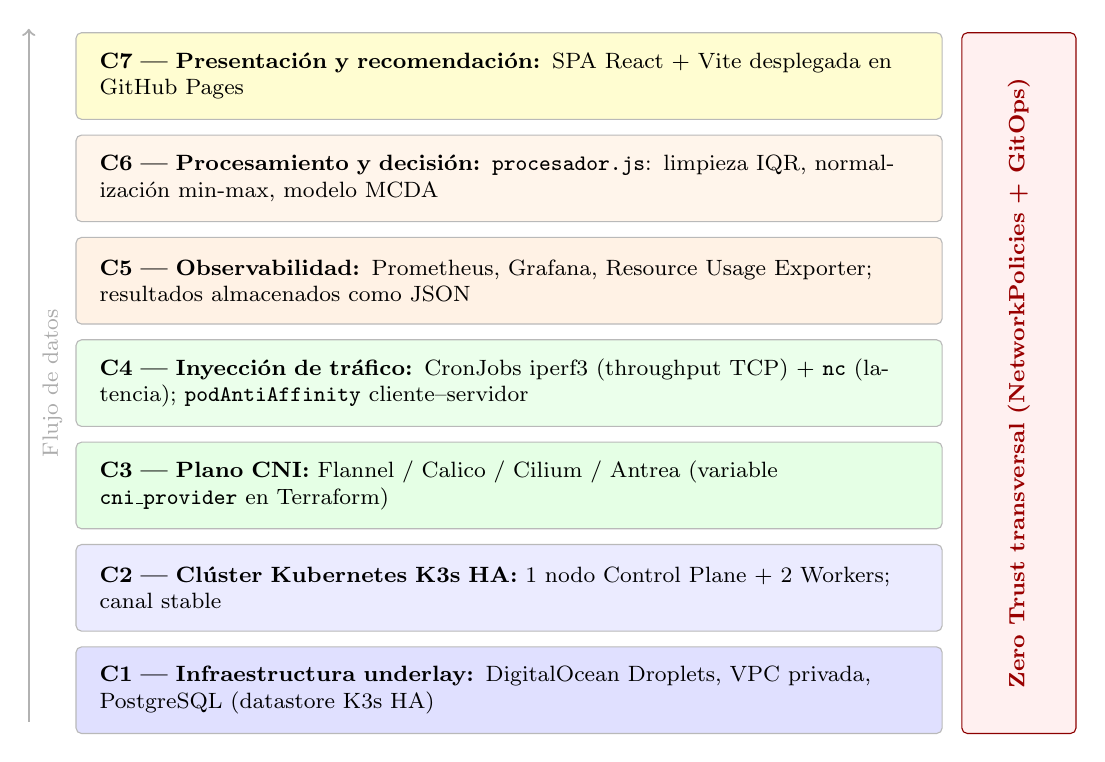
\begin{tikzpicture}[font=\footnotesize]
\tikzset{lay/.style={draw=gray!55, minimum width=11cm, minimum height=1.1cm,
    text width=10.4cm, align=left, inner sep=4pt, rounded corners=2pt}}

\node[lay, fill=blue!12] at (0,0.0)
    {\textbf{C1 --- Infraestructura underlay:} DigitalOcean Droplets, VPC privada, PostgreSQL (datastore K3s HA)};
\node[lay, fill=blue!8] at (0,1.3)
    {\textbf{C2 --- Clúster Kubernetes K3s HA:} 1 nodo Control Plane + 2 Workers; canal stable};
\node[lay, fill=green!10] at (0,2.6)
    {\textbf{C3 --- Plano CNI:} Flannel / Calico / Cilium / Antrea (variable \texttt{cni\_provider} en Terraform)};
\node[lay, fill=green!8] at (0,3.9)
    {\textbf{C4 --- Inyección de tráfico:} CronJobs iperf3 (throughput TCP) + \texttt{nc} (latencia); \texttt{podAntiAffinity} cliente--servidor};
\node[lay, fill=orange!10] at (0,5.2)
    {\textbf{C5 --- Observabilidad:} Prometheus, Grafana, Resource Usage Exporter; resultados almacenados como JSON};
\node[lay, fill=orange!8] at (0,6.5)
    {\textbf{C6 --- Procesamiento y decisión:} \texttt{procesador.js}: limpieza IQR, normalización min-max, modelo MCDA};
\node[lay, fill=yellow!18] at (0,7.8)
    {\textbf{C7 --- Presentación y recomendación:} SPA React + Vite desplegada en GitHub Pages};

% Zero Trust transversal bar
\fill[red!6, draw=red!55!black, rounded corners=2pt] (5.75,-0.55) rectangle (7.20,8.35);
\node[rotate=90, font=\footnotesize\bfseries, text=red!60!black] at (6.475,3.90)
    {Zero Trust transversal (NetworkPolicies + GitOps)};

% Data flow arrow
\draw[->, thick, gray!60] (-6.10,-0.40) -- (-6.10,8.40);
\node[rotate=90, font=\footnotesize, text=gray!65] at (-5.80,3.90) {Flujo de datos};

\end{tikzpicture}
\caption{Arquitectura por capas del testbed experimental.}
\label{fig:arquitectura-capas}
\end{figure}
\shorthandon{>}

\subsection{Trazabilidad y Requisitos de Diseño}

El diseño no se planteó como una arquitectura aislada, sino como respuesta directa al problema formulado en el anteproyecto: las organizaciones adoptan Kubernetes como plataforma de orquestación, pero la calidad final del despliegue depende del plano de red, de la selección del CNI y del control de las comunicaciones internas del clúster \cite{ref29}. La Tabla~\ref{tab:trazabilidad-diseno} hace explícita la correspondencia entre cada necesidad, su objetivo asociado y la decisión de diseño que la atiende.

\begin{table}[htbp]
\centering
\scriptsize
\caption{Trazabilidad entre problema de investigación, objetivo y decisión de diseño.}
\label{tab:trazabilidad-diseno}
\begin{tabularx}{\textwidth}{|Y|Y|Y|}
\hline
\textbf{Necesidad identificada} & \textbf{Objetivo asociado} & \textbf{Respuesta de diseño} \\
\hline
Comparar CNIs sin depender de recomendaciones informales. & Evaluar cuantitativamente Calico, Cilium, Flannel y Antrea en escenarios controlados. & Testbed reproducible sobre Kubernetes, ejecución automatizada y consolidación de métricas por CNI. \\
\hline
Controlar el riesgo de comunicaciones internas abiertas. & Evaluar políticas de red seguras y automatizadas. & NetworkPolicies bajo enfoque Zero Trust, casos de denegación por defecto y segmentación por capas. \\
\hline
Convertir resultados técnicos heterogéneos en una decisión comprensible. & Definir criterios, umbrales y ponderaciones para comparación objetiva. & Modelo MCDA con criterios de rendimiento, eficiencia de recursos e impacto de seguridad. \\
\hline
Apoyar a una organización que necesita seleccionar y configurar un CNI. & Implementar un prototipo funcional de recomendación. & Prototipo web que consume datos procesados, aplica perfiles de decisión y explica la recomendación. \\
\hline
Evitar sobredimensionamiento de infraestructura. & Relacionar desempeño de red con consumo de CPU y memoria. & Captura de recursos del CNI mediante Prometheus y cálculo de eficiencia relativa por perfil. \\
\hline
\end{tabularx}
\end{table}

De este planteamiento se derivan cinco requisitos de diseño. La \textbf{reproducibilidad} se obtiene mediante infraestructura como código, despliegue declarativo y automatización de experimentos. El \textbf{aislamiento de variables} mantiene constante todo elemento distinto del CNI ---proveedor, tipo de instancia, versión de Kubernetes, topología y duración---. La \textbf{medición integral} evalúa el CNI por rendimiento de red, eficiencia de recursos e impacto de seguridad, y no solo por throughput. La \textbf{trazabilidad de la evidencia} exige que cada dato conserve su origen. La \textbf{compatibilidad con la operación real} se logra empleando objetos y patrones nativos de Kubernetes ---Deployments, CronJobs, ArgoCD--- cercanos a la práctica de los equipos de operaciones.

\subsection{Prototipo Recomendador}

El prototipo recomendador es la capa de interacción entre el modelo matemático y el usuario final. Su salida comprende tres niveles: la recomendación directa (qué CNI se sugiere), la justificación (qué métricas la explican) y la orientación de configuración (qué consideraciones debe atender el usuario al desplegar ese CNI), estructura que responde al objetivo específico 4 del anteproyecto \cite{ref29}. Se implementó como SPA con React~19, Vite~7 y Tailwind CSS~3; el \emph{build} de producción se despliega en GitHub Pages, y la actualización de datos encadena \texttt{procesador.js} ---que genera \texttt{cni-data.json}--- con la inyección de esos datos en el \emph{bundle}.

\subsection{Alcance y Límites del Diseño}

El diseño se limita a evaluar CNIs en un testbed controlado sobre Kubernetes y no pretende generalizar automáticamente los resultados a cualquier proveedor, versión o hardware. Emplea tráfico TCP controlado como señal principal y no asume que una mayor complejidad implique un mejor resultado. La solución se concibió para sostener una mejora continua: a medida que se incorporen nuevas corridas o versiones de CNIs, el pipeline puede recalcular los puntajes. En lugar de entregar una decisión congelada, ofrece un método para decidir con evidencia actualizable: técnicamente, reemplaza opiniones por datos medidos en condiciones reproducibles; económicamente, conocer el consumo de CPU de cada CNI por unidad de tráfico permite dimensionar la infraestructura sin márgenes precautorios excesivos \cite{ref29}.

\section{Implementación de la Solución}

La infraestructura está codificada en Terraform, la configuración en manifiestos YAML versionados en Git y las pruebas automatizadas en CronJobs de Kubernetes ---condición necesaria para que los resultados sean reproducibles y atribuibles al CNI \cite{ref7}.

\subsection{Aprovisionamiento de Infraestructura con Terraform}

El aprovisionamiento de servidores y redes se realizó mediante Terraform (IaC). Al describir la infraestructura en archivos versionados, Terraform la recrea de manera idéntica en cada ejecución y elimina la posibilidad de que variaciones manuales introduzcan diferencias entre los entornos de cada CNI \cite{ref7}.

\subsubsection{Estructura del Código Terraform (K8s-bootstrap/00.bootstrap)}

\begin{table}[htbp]
\centering
\scriptsize
\renewcommand{\arraystretch}{1.25}
\setlength{\tabcolsep}{4pt}
\caption{Archivos Terraform del módulo de aprovisionamiento y su función específica.}
\label{tab:terraform-aprovisionamiento}
\begin{tabularx}{\textwidth}{|l|Y|}
\hline
\textbf{Archivo Terraform} & \textbf{Responsabilidad en la Infraestructura} \\
\hline
\texttt{main.tf} & Define los recursos principales: Droplets de DigitalOcean y red VPC privada. \\
\hline
\texttt{variables.tf} & Centraliza todos los parámetros configurables: número de nodos (\texttt{agent\_count = 2}), tamaño de instancias, región y proveedor CNI. \\
\hline
\texttt{ssh\_keys.tf} & Automatiza la gestión de llaves SSH para el acceso seguro entre nodos. \\
\hline
\texttt{firewall.tf} & Configura las reglas de firewall a nivel de nube: primera línea de seguridad perimetral. \\
\hline
\texttt{outputs.tf} & Genera automáticamente el archivo kubeconfig con las credenciales del clúster K3s. \\
\hline
\end{tabularx}
\end{table}

El proceso de aprovisionamiento tiene tres etapas: \texttt{terraform plan} (compara estado actual vs. código), \texttt{terraform apply} (crea Droplets, VPC y firewall) y \texttt{terraform output} (extrae IPs y kubeconfig). Terraform mantiene un archivo \texttt{terraform.tfstate} que permite destruir y recrear toda la infraestructura de manera controlada, garantizando la repetibilidad científica: cada CNI se evaluó en condiciones idénticas de arranque.

\subsection{Configuración del Clúster K3s en Alta Disponibilidad}

Una vez aprovisionados los servidores, se instaló y configuró K3s, una distribución liviana de Kubernetes, con topología de 1 nodo Master + 2 nodos Worker dedicados.

\subsubsection{Base de Datos Externa para el Plano de Control}

El plano de control se configuró con una base de datos PostgreSQL gestionada de DigitalOcean (también provisionada via Terraform) como datastore externo. Esto elimina la complejidad de mantener un clúster etcd y garantiza un plano de control sin punto único de fallo (SPOF).

\subsubsection{Instalación: clúster sin CNI para plugins externos y modo nativo para Flannel}

La implementación establece una distinción metodológica deliberada: Flannel se evalúa en su modo de despliegue más habitual ---integrado nativamente en K3s con \texttt{flannel-iface: eth1}---, mientras que Calico, Cilium y Antrea se instalan como plugins externos sobre un clúster sin CNI. La asimetría refleja las condiciones reales de uso: Flannel es el CNI predeterminado de K3s y la mayoría de equipos lo adopta sin configuración adicional, en tanto que los otros tres requieren instalación explícitamente y de forma declarativa. Evaluar cada CNI en su escenario de despliegue típico aumenta la validez ecológica del experimento~\cite{ref7}; debe considerarse, no obstante, que Flannel se beneficia de la integración nativa de K3s ---gestión automática de CIDR y \emph{hooks} de kubelet--- que los plugins externos deben replicar por su cuenta.

Para los CNIs externos, la configuración crítica es el parámetro \texttt{--flannel-backend=none}, que desactiva completamente el CNI integrado de K3s y evita interferencias con el plugin bajo evaluación. Adicionalmente, se configura \texttt{--disable-network-policy} para que K3s no intente implementar NetworkPolicies por sí mismo.

La configuración resultante en \texttt{/etc/rancher/k3s/config.yaml} para CNIs externos incluye:
\begin{lstlisting}
flannel-backend: none
disable-network-policy: true
\end{lstlisting}

\begin{table}[htbp]
\centering
\scriptsize
\renewcommand{\arraystretch}{1.25}
\setlength{\tabcolsep}{4pt}
\caption{Instalación de CNIs: método y configuración clave en \texttt{user\_data/ks3\_server\_init.sh}.}
\label{tab:cni-instalacion}
\begin{tabularx}{\textwidth}{|l|p{3.2cm}|Y|}
\hline
\textbf{CNI} & \textbf{Método de instalación} & \textbf{Configuración clave} \\
\hline
Flannel & Nativo K3s & \texttt{flannel-iface: eth1} (interfaz VPC de DigitalOcean) \\
\hline
Calico & Tigera Operator v3.29.1 & \texttt{encapsulation: VXLAN}, CIDR \texttt{10.42.0.0/16}, \texttt{nodeAddressAutodetectionV4.interface: eth1} \\
\hline
Cilium & Helm 1.16.5 & \texttt{routingMode=tunnel}, \texttt{tunnelProtocol=vxlan}, \texttt{ipam.mode=kubernetes}, \texttt{devices=eth1}, \texttt{operator.replicas=1} \\
\hline
Antrea & Manifest v2.2.0 & \texttt{transportInterface: eth1}, \texttt{serviceCIDR: 10.43.0.0/16} \\
\hline
\end{tabularx}
\end{table}

El protocolo de rotación de CNIs se implementó mediante el reemplazo completo de la infraestructura entre ciclos. Para cambiar de un CNI al siguiente, se modificó la variable \texttt{cni\_provider} en \texttt{terraform.tfvars} y se ejecutó \texttt{terraform destroy} seguido de \texttt{terraform apply}: el primero eliminó todos los recursos de DigitalOcean (Droplets, VPC y base de datos PostgreSQL), y el segundo los recreó desde cero con el nuevo CNI preconfigurado en el script de inicialización de K3s. Este enfoque garantiza que cada ciclo de prueba parte de nodos completamente limpios, sin residuos de configuración del CNI anterior que pudieran contaminar las métricas.

\subsection{Orquestación y Entrega Continua: GitOps con ArgoCD}

Con el clúster K3s funcionando y sin CNI, el siguiente componente instalado fue ArgoCD. ArgoCD implementa el paradigma GitOps: el repositorio Git es la única fuente de verdad sobre el estado del clúster. Todo lo que debe existir en el clúster está definido en archivos YAML dentro del repositorio \texttt{K8s-Tesis-Apps}. Esta centralización en Git facilita la auditoría del experimento: cualquier cambio en la configuración queda registrado con autor, fecha y motivo, haciendo el proceso de prueba completamente trazable.

\subsubsection{El Patrón App of Apps}

La implementación de ArgoCD utiliza el patrón App of Apps: existe UNA sola aplicación raíz (ubicada en \texttt{K8s-bootstrap/30.apps-of-apps-install}) que ArgoCD conoce directamente, y esa aplicación raíz contiene las definiciones de todas las demás aplicaciones (CNIs, stack de métricas, benchmarks, políticas de red).

\subsubsection{Configuración de selfHeal y prune}

\textbf{\emph{selfHeal: true}} --- Ante la modificación manual de un recurso del clúster ---por ejemplo, la eliminación de una NetworkPolicy---, ArgoCD detecta la diferencia con el repositorio Git y restaura el estado original, lo que resultó crítico para la integridad del experimento.

\textbf{\emph{prune: true}} --- Al eliminar un archivo YAML del repositorio Git, ArgoCD elimina también el recurso correspondiente del clúster, lo que evita la acumulación de recursos huérfanos.

\begin{lstlisting}
# Definicion de la Application raiz en ArgoCD (App of Apps)
apiVersion: argoproj.io/v1alpha1
kind: Application
metadata:
  name: apps-of-apps
  namespace: argocd
spec:
  source:
    repoURL: https://github.com/equipo/K8s-Tesis-Apps
    targetRevision: main
    path: apps/
  syncPolicy:
    automated:
      selfHeal: true   # Restaura cambios manuales automaticamente
      prune: true      # Elimina recursos borrados del repo
\end{lstlisting}

\subsubsection{Overlays de Kustomize para los CNIs}

Cada CNI tiene una configuración ligeramente diferente. Para gestionarlas sin duplicar código, se utilizó Kustomize con el patrón base/overlay: existe una configuración base con los parámetros comunes, y sobre esa base se aplican overlays específicas para cada CNI.

Las apps gestionadas por ArgoCD include: \texttt{cni-test-iperf} (benchmarks de throughput y latencia), \texttt{cni-resource-exporter} (exportación de recursos desde Prometheus), \texttt{cni-np-test} (pruebas de Network Policies, creada solo cuando \texttt{cni\_provider != "flannel"} y el caso de uso está definido), y \texttt{metrics} (Prometheus + Grafana).

\subsection{Implementación del Stack de Observabilidad}

El stack de observabilidad se implementó mediante el \texttt{kube-prometheus-stack} (Helm chart) que instala Prometheus, Grafana y exportadores preconfigurados para Kubernetes.

\subsubsection{Prometheus: El Recolector de Métricas}

Prometheus opera con un modelo pull: visita periódicamente los endpoints de métricas (cada 15 segundos en la configuración del proyecto). Para que Prometheus sepa qué métricas recolectar de los agentes CNI, se implementaron \texttt{ServiceMonitors} (CRD), apuntando específicamente al endpoint de métricas de cada agente. Un intervalo de 15 segundos proporciona suficiente granularidad para detectar picos de consumo durante las ráfagas de tráfico iperf3, sin generar una carga de scraping que interfiera con las métricas bajo observación.

Las métricas clave recolectadas del agente CNI incluyen:
\begin{itemize}
\item \path|container_cpu_usage_seconds_total| (filtrado por pod del agente): costo computacional del CNI (criterio C2 del marco MCDA).
\item \path|container_memory_rss| (filtrado por pod del agente): memoria física real del proceso del agente CNI.
\item \path|node_network_transmit_bytes_total| / \path|node_network_receive_bytes_total|: bytes totales de red por nodo.
\item \path|kube_pod_info| + \path|kube_pod_status_phase|: estado del agente CNI para detectar reinicios durante las pruebas.
\end{itemize}

\subsubsection{Grafana: Los Dashboards de Red}

Grafana centraliza la lectura operativa de las series de Prometheus. Sus paneles agrupan throughput, latencia, consumo del agente CNI y score MCDA. Esta correlación vincula ráfagas iperf3 con CPU, RSS y el ranking calculado por \texttt{procesador.js}.

\subsubsection{Resource Usage Exporter: Extracción Automatizada de Datos}

El \texttt{cni-resource-usage-exporter} corre como CronJob en \path|K8s-Tesis-Apps/grafana-exporter|. ArgoCD sincroniza el recurso mediante la app \texttt{cni-resource-exporter}. El CronJob:
\begin{itemize}
\item Ejecuta la extracción en los minutos 25 y 55 de cada hora, tras cada ventana de benchmarks.
\item Consulta directamente la API HTTP de Prometheus (\texttt{/api/v1/query\_range}) --- no interactúa con Grafana.
\item Recolecta CPU\% por nodo, RAM\% por nodo, RAM usada, CPU cores y RAM del agente CNI.
\item Genera \texttt{raw/}, \texttt{csv/}, \texttt{images/} y \texttt{cni\_resource\_summary.json} por corrida.
\item Persiste cada salida con timestamp en \path|K8S-CNI-Results/results/cni-benchmarks/{cni}/resource_usage_nodes/|.
\end{itemize}

\subsection{Implementación del Banco de Pruebas de QoS}

\subsubsection{Escenario de Rendimiento con iperf3}

El banco de throughput se define en \texttt{K8s-Tesis-Apps/cni\_test\_iperf}:

\textbf{El iperf3-server (Deployment):} Un Deployment ejecuta una réplica de iperf3 en modo servidor. Un Service ClusterIP expone un nombre DNS estable para el cliente.

\textbf{El iperf3-client (CronJob):} La programación \texttt{0,30 * * * *} activa el cliente en los minutos 0 y 30. \texttt{concurrencyPolicy: Forbid} bloquea corridas simultáneas. Cada activación crea un Pod y genera tráfico TCP durante 300 segundos. La salida conserva formato JSON con \texttt{iperf3 -t 300 -i 10 -J}. La retención máxima queda en 5 corridas (\texttt{RETENTION\_MAX\_RUNS="5"}).

La anti-afinidad del cliente frente al servidor se implementó como \texttt{preferredDuringSchedulingIgnoredDuringExecution} (suave, weight 100), forzando tráfico inter-nodo en la práctica. Esta ubicación garantiza que todo el tráfico de benchmark atraviese el mecanismo de encapsulación del CNI entre nodos, que es exactamente lo que se quiere medir.

\begin{lstlisting}
# iperf-client-cronjob.yaml -- fragmento relevante
schedule: '0,30 * * * *'   # Minutos 0 y 30
concurrencyPolicy: Forbid
affinity:
  podAntiAffinity:
    preferredDuringSchedulingIgnoredDuringExecution:
    - weight: 100
      podAffinityTerm:
        labelSelector:
          matchLabels:
            app: iperf-server
        topologyKey: kubernetes.io/hostname
# iperf3 -c iperf-server-svc -t 300 -i 10 -J
\end{lstlisting}

\subsubsection{Cliente de Latencia Personalizado}

El CronJob \texttt{latency-client-cronjob.yaml} ejecuta la prueba de latencia. Su programación corre en los minutos 10 y 40 de cada hora. Esa separación evita solapamiento con el inicio del throughput.

El cliente registra TCP Connect con \texttt{nc -z -w 2} y timestamp en ms. Cada corrida toma 30 muestras y calcula min/avg/max/mdev. El JSON normalizado conserva campos de latencia, muestras intentadas y muestras exitosas.

\begin{table}[htbp]
\centering
\scriptsize
\renewcommand{\arraystretch}{1.25}
\setlength{\tabcolsep}{4pt}
\caption{Métricas de QoS capturadas por el banco de pruebas y su relevancia telemática.}
\label{tab:metricas-qos-implementacion}
\begin{tabularx}{\textwidth}{|p{4cm}|p{2.4cm}|Y|}
\hline
\textbf{Métrica Capturada} & \textbf{Unidad} & \textbf{Relevancia para QoS Telemático} \\
\hline
Throughput TCP sostenido & Gbps / Mbps & Capacidad efectiva de la red. \\
\hline
Latencia mínima TCP connect & ms & Overhead mínimo del CNI sin congestión. \\
\hline
Latencia promedio TCP connect & ms & Comportamiento típico de solicitudes. \\
\hline
Latencia máxima / Jitter & ms & Peor caso y variabilidad. Crítico para tiempo real. \\
\hline
Retransmisiones TCP & count / sesión & Indicador de problemas en encapsulamiento o congestión. \\
\hline
CPU del agente CNI & millicores (m) & Impacto directo en costo de infraestructura cloud. \\
\hline
RAM del agente CNI (RSS) & MiB & Huella de memoria del agente CNI por nodo. \\
\hline
\end{tabularx}
\end{table}

\subsection{Procesamiento Estadístico y Aplicación del Modelo MCDA}

\subsubsection{Limpieza con el Rango Intercuartílico (IQR)}

\texttt{docs/procesador.js} transforma datos crudos en datos consolidados. El script descubre los CNIs disponibles bajo \texttt{results/cni-benchmarks}. Luego extrae métricas desde JSON y CSV. Finalmente aplica IQR:

\begin{lstlisting}
// procesador.js -- Funcion de limpieza estadistica IQR
function calcularEstadisticasLimpias(valores) {
  const sorted = [...valores].sort((a, b) => a - b);
  const q1 = sorted[Math.floor(sorted.length * 0.25)];
  const q3 = sorted[Math.floor(sorted.length * 0.75)];
  const iqr = q3 - q1;
  const lowerBound = q1 - 1.5 * iqr;
  const upperBound = q3 + 1.5 * iqr;
  const valoresLimpios = valores.filter(
    v => v >= lowerBound && v <= upperBound);
  const promedio = valoresLimpios.reduce(
    (sum, v) => sum + v, 0) / valoresLimpios.length;
  return { promedio,
    outliersPorcentaje: ((valores.length - valoresLimpios.length)
      / valores.length * 100).toFixed(1)
  };
}
\end{lstlisting}

El pipeline descarta valores atípicos antes de calcular promedios. Dado que un evento cloud anómalo puede sesgar una corrida, el filtro estabiliza el puntaje MCDA del CNI.

\subsubsection{Normalización y Cálculo del Score MCDA}

Después de la limpieza, el pipeline aplica la normalización min-max re-escalada a $[1,\,5]$ descrita en el Marco Teórico. En métricas positivas como throughput, la normalización es directa ($V_i = 5$ al máximo). En métricas negativas como latencia o CPU, el cociente se invierte, de modo que el valor más bajo recibe $V_i = 5$ y el más alto $V_i = 1$. La escala uniforme permite comparar Gbps, milisegundos y millicores sin sesgo por magnitud numérica.

\begin{lstlisting}
// recommendationModel.js -- Calculo del overhead de seguridad
function getNetworkPolicyOverhead(data) {
  if (!data?.network_policy) return null;
  const caseValues = Object.values(data.network_policy).flatMap(
    (policyCase) => [
      Number(policyCase?.overhead_latencia_pct),
      Number(policyCase?.overhead_throughput_pct),
  ]);
  const validValues = caseValues.filter((v) => Number.isFinite(v));
  if (!validValues.length) return null;
  return average(validValues);
}
// El score de seguridad se invierte (menor overhead = 5.0).
// Si meta.supportsNetworkPolicy === false (ej. Flannel), el score es 1.
\end{lstlisting}

El pipeline calcula el puntaje de la dimensión de seguridad evaluando el impacto (\emph{overhead}) promedio en latencia y throughput al activar los casos de prueba de \texttt{network\_policy}. Entre menor sea la degradación del rendimiento al aislar los Pods, mayor será la calificación normalizada del CNI. Aquellos plugins que por diseño no implementan Network Policies en su plano de datos reciben por defecto la calificación mínima de $1.00$ en esta dimensión, penalizando su uso en entornos que requieran aislamiento lógico.

\subsection{Prototipo Recomendador: Aplicación Web SPA}

\subsubsection{Tecnologías de Implementación}

La SPA fue implementada con React~19 (gestión de estado por componentes), Vite~7 (bundler; build de producción vía \texttt{build:pages} con \texttt{--outDir ../docs/recommender}) y Tailwind CSS~3 (estilos utilitarios directamente en JSX, sin CSS personalizado).

\texttt{npm run sync:data} ejecuta \texttt{procesador.js} y genera \texttt{cni-data.json}. Después, \texttt{export-spa-data.cjs} inyecta los datos en el bundle. \texttt{recommendationModel.js} concentra la lógica de recomendación.

\subsubsection{Flujo de la Aplicación}

\begin{enumerate}
\item \textbf{Selección de Perfil:} La pantalla principal muestra tres tarjetas: Fintech/Seguridad, Streaming/Rendimiento e IoT/Recursos.
\item \textbf{Visualización de Resultados:} La aplicación carga \texttt{cni-data.json} y calcula el ranking MCDA para el perfil seleccionado. El CNI con mayor puntaje queda marcado como recomendación.
\item \textbf{Justificación Técnica:} La interfaz expone las métricas brutas promedio de cada CNI en gráficas comparativas.
\end{enumerate}

\subsection{Implementación de Network Policies y Seguridad Zero Trust}

\subsubsection{Políticas Default Deny}

Default Deny operacionaliza el modelo Zero Trust. La política bloquea todo el tráfico inicial y habilita solo comunicaciones necesarias. Con esta regla, toda comunicación no autorizada falla sin intervención del operador.

El siguiente manifiesto aplica la política a todos los Pods del namespace \texttt{production}:

\begin{lstlisting}
# default-deny-all.yaml
apiVersion: networking.k8s.io/v1
kind: NetworkPolicy
metadata:
  name: default-deny-all
  namespace: production
spec:
  podSelector: {}     # aplica a TODOS los Pods del namespace
  policyTypes:
  - Ingress           # Bloquea todo el trafico entrante
  - Egress            # Bloquea todo el trafico saliente
\end{lstlisting}

\subsubsection{Micro-segmentación por Capas de Aplicación}

Sobre Default Deny, las políticas específicas acotan el tráfico permitido. Las reglas \texttt{frontend $\rightarrow$ backend $\rightarrow$ database} usan label selectors.

En Cilium, una \texttt{CiliumNetworkPolicy} de capa 7 admite solo métodos \texttt{GET} y \texttt{HEAD} desde frontend hacia backend. En Antrea, una \texttt{ClusterNetworkPolicy} en el Tier \texttt{securityops} prioriza sobre cualquier \texttt{NetworkPolicy} de namespace.

Esta estratificación evalúa seguridad granular en condiciones reales. También cuantifica si esa granularidad introduce overhead detectable, uno de los criterios del modelo MCDA.

\subsubsection{Validación Automatizada de Políticas}

Se implementó un pipeline de validación que emplea \texttt{nc} (netcat) dentro de Pods de prueba para verificar la conectividad. Para cada par de Pods, el pipeline define una expectativa ---la conexión debe permitirse o debe bloquearse--- y reporta un error cuando el comportamiento observado no coincide con ella.

\begin{table}[htbp]
\centering
\scriptsize
\renewcommand{\arraystretch}{1.25}
\setlength{\tabcolsep}{4pt}
\caption{Casos de prueba del pipeline de validación de Network Policies.}
\label{tab:validacion-network-policies}
\begin{tabularx}{\textwidth}{|p{5cm}|Y|}
\hline
\textbf{Prueba de Validación} & \textbf{Resultado Esperado y Justificación} \\
\hline
frontend $\rightarrow$ backend (puerto 8080) & PERMITIDO --- Comunicación necesaria para el funcionamiento de la aplicación. \\
\hline
frontend $\rightarrow$ database (puerto 5432) & BLOQUEADO --- El frontend no debe acceder directamente a la base de datos. \\
\hline
backend $\rightarrow$ database (puerto 5432) & PERMITIDO --- El backend necesita leer y escribir datos. \\
\hline
database $\rightarrow$ cualquier Pod & BLOQUEADO --- La base de datos nunca debe iniciar conexiones salientes. \\
\hline
Pod externo $\rightarrow$ namespace production & BLOQUEADO --- Sin una regla explícita, ningún Pod externo puede entrar. \\
\hline
\end{tabularx}
\end{table}

\subsection{Estructura de Repositorios y Entregables Técnicos}

La Tabla~\ref{tab:repositorios-entregables} resume la organización del proyecto en tres repositorios Git.

\begin{table}[htbp]
\centering
\scriptsize
\renewcommand{\arraystretch}{1.25}
\setlength{\tabcolsep}{4pt}
\caption{Estructura de los cuatro repositorios del proyecto y su relación con los objetivos específicos.}
\label{tab:repositorios-entregables}
\begin{tabularx}{\textwidth}{|p{3cm}|Y|p{5.2cm}|}
\hline
\textbf{Repositorio} & \textbf{Contenido Principal} & \textbf{Relación con los Objetivos} \\
\hline
\texttt{HA-K3s-Terraform-DO} & Módulo Terraform reutilizable que provisiona Droplets, VPC, Load Balancer y base de datos PostgreSQL en DigitalOcean. & OE1: Módulo base de infraestructura cloud invocado por \texttt{K8s-bootstrap}. \\
\hline
\texttt{K8s-bootstrap} & Código Terraform (\texttt{00.bootstrap}), scripts de instalación K3s HA (\texttt{10.k3s-ha-do}), manifiestos de ArgoCD (\texttt{20.argo-cd-install}) y App of Apps (\texttt{30.apps-of-apps-install}). & OE1: Orquesta el aprovisionamiento completo del testbed. \\
\hline
\texttt{K8s-Tesis-Apps} & Overlays Kustomize para los 4 CNIs, stack de observabilidad (\texttt{apps/metrics}), benchmarks iperf3 (\texttt{cni\_test\_iperf}), cliente de latencia, Network Policies y Grafana Exporter. & OE1, OE2 y OE3: Implementa las pruebas, la seguridad y el sistema de recolección. \\
\hline
\texttt{K8S-CNI-Results} & Archivos JSON/CSV con resultados por corrida, \texttt{procesador.js} (modelo MCDA) y la SPA recomendadora (\texttt{cni-recommender-spa}). & OE3 y OE4: Implementa el modelo de comparación objetiva y el prototipo. \\
\hline
\end{tabularx}
\end{table}

La arquitectura mantiene un flujo unidireccional: \texttt{HA-K3s-Terraform-DO} provee el módulo cloud; \texttt{K8s-bootstrap} orquesta la infraestructura; \texttt{K8s-Tesis-Apps} despliega las aplicaciones y genera métricas; \texttt{K8S-CNI-Results} almacena, procesa y visualiza resultados.

\subsection{Desafíos de Implementación y Soluciones Adoptadas}

\begin{table}[htbp]
\centering
\scriptsize
\renewcommand{\arraystretch}{1.25}
\setlength{\tabcolsep}{4pt}
\caption{Desafíos técnicos encontrados durante la implementación y soluciones adoptadas.}
\label{tab:desafios-implementacion}
\begin{tabularx}{\textwidth}{|Y|Y|}
\hline
\textbf{Desafío Encontrado} & \textbf{Solución Técnica Implementada} \\
\hline
MTU mismatch al instalar Cilium: Pods no podían comunicarse, paquetes se fragmentaban silenciosamente en la VPC. Flannel y Calico detectan automáticamente la MTU de la interfaz subyacente en sus versiones actuales; Cilium requirió configuración explícita porque su dataplane eBPF no hereda el valor de MTU del sistema operativo sin intervención. & Se calculó la MTU efectiva: 1500 (VPC) $-$ 50 (overhead VXLAN) $=$ 1450. Se configuró el parámetro \texttt{mtu: 1450} en el overlay de Kustomize de Cilium. \\
\hline
ArgoCD en estado OutOfSync al instalar el stack de métricas (Prometheus + Grafana): los CRDs del \texttt{kube-prometheus-stack} se aplicaban en el mismo ciclo de sync que los recursos que los consumían, provocando fallo en el despliegue porque el API server aún no conocía los tipos personalizados. & Se separó la instalación en dos Applications independientes usando sync waves: \texttt{kube-prometheus-stack-crds} (wave~$-1$) despliega el mismo chart con todos los componentes deshabilitados ---solo crea los CRDs--- usando \texttt{ServerSideApply=true}; \texttt{kube-prometheus-stack} (wave~$0$) despliega el stack completo con \texttt{skipCrds:~true} y \texttt{SkipDryRunOnMissingResource=true}, garantizando que los CRDs existen antes de crear los recursos dependientes. \\
\hline
Outliers frecuentes en pruebas de madrugada: DigitalOcean mostraba throttling de CPU en horas de alta demanda del datacenter. & Se configuró una ventana de pruebas exclusiva para horario laboral. El algoritmo IQR filtra automáticamente estos outliers. \\
\hline
\texttt{procesador.js} necesitaba evaluar la seguridad de forma cuantitativa e integrada en el MCDA, pero Flannel no reportaba overhead al no soportar políticas. & Se parametrizó el score de seguridad basándose en el overhead de latencia de las políticas. Para los CNIs que no soportan políticas (Flannel), el modelo asigna directamente el puntaje mínimo de $1.0$ en la dimensión de seguridad. \\
\hline
\end{tabularx}
\end{table}

\subsection{Flujo completo de ejecución}

El flujo integral de cinco etapas ---generación de tráfico, captura de métricas, extracción de recursos, scoring MCDA y visualización--- se describió en la sección~\ref{sec:Metodos} e ilustra en la Figura~\ref{fig:arquitectura-capas}. En conjunto, los cuatro repositorios implementan ese flujo de forma unidireccional y reproducible.